\documentclass{article}

\usepackage{mathtools}
\usepackage{graphicx}
\usepackage{listings}
\usepackage{color}

\definecolor{mygreen}{rgb}{0,0.6,0} 
\definecolor{mygray}{rgb}{0.5,0.5,0.5} 
\definecolor{mymauve}{rgb}{0.58,0,0.82}

%Scala
\lstdefinelanguage{scala}{
  morekeywords={abstract,case,catch,class,def,%
    do,else,extends,false,final,finally,%
    for,if,implicit,import,match,mixin,%
    new,null,object,override,package,%
    private,protected,requires,return,sealed,%
    super,this,throw,trait,true,try,%
    type,val,var,while,yield},
  otherkeywords={=>,<-,<\%,<:,>:,\#,@},
  sensitive=true,
  morecomment=[l]{//},
  morecomment=[n]{/*}{*/},
  morestring=[b]",
  morestring=[b]',
  morestring=[b]"""
}

% Default settings for code listings
\lstset{frame=tb,
  language=scala,
  aboveskip=3mm,
  belowskip=3mm,
  showstringspaces=false,
  columns=flexible,
  basicstyle={\small\ttfamily},
  numbers=none,
  numberstyle=\tiny\color{mygray},
  keywordstyle=\color{blue},
  commentstyle=\color{mygreen},
  stringstyle=\color{mymauve},
  frame=single,
  breaklines=true,
  breakatwhitespace=true
  tabsize=3
}

\title{Dissertation proposal - Metrics for code 'functional-ness' in Scala }
\date{\today}

\begin{document}



\pagenumbering{gobble}
\maketitle

\vspace{30mm} %5mm vertical space

\begin{center}
Master Student Name: Alexandru Matei \par
Supervisor Name : Marius Minea \par
Dissertation Domain: Software engineering - Functional Programming
\end{center}

\vfill

\newpage
\tableofcontents
\newpage

\pagenumbering{arabic}
\section{Introduction}
Functional programming started to get more traction in the last years, thanks to the growing adoption of Scala and Haskell in the software industry; we can see that Google trends shows a rising interest in functional programming languages (see figure \ref{fig:google-rank}). \par

\begin{figure}[h!]
  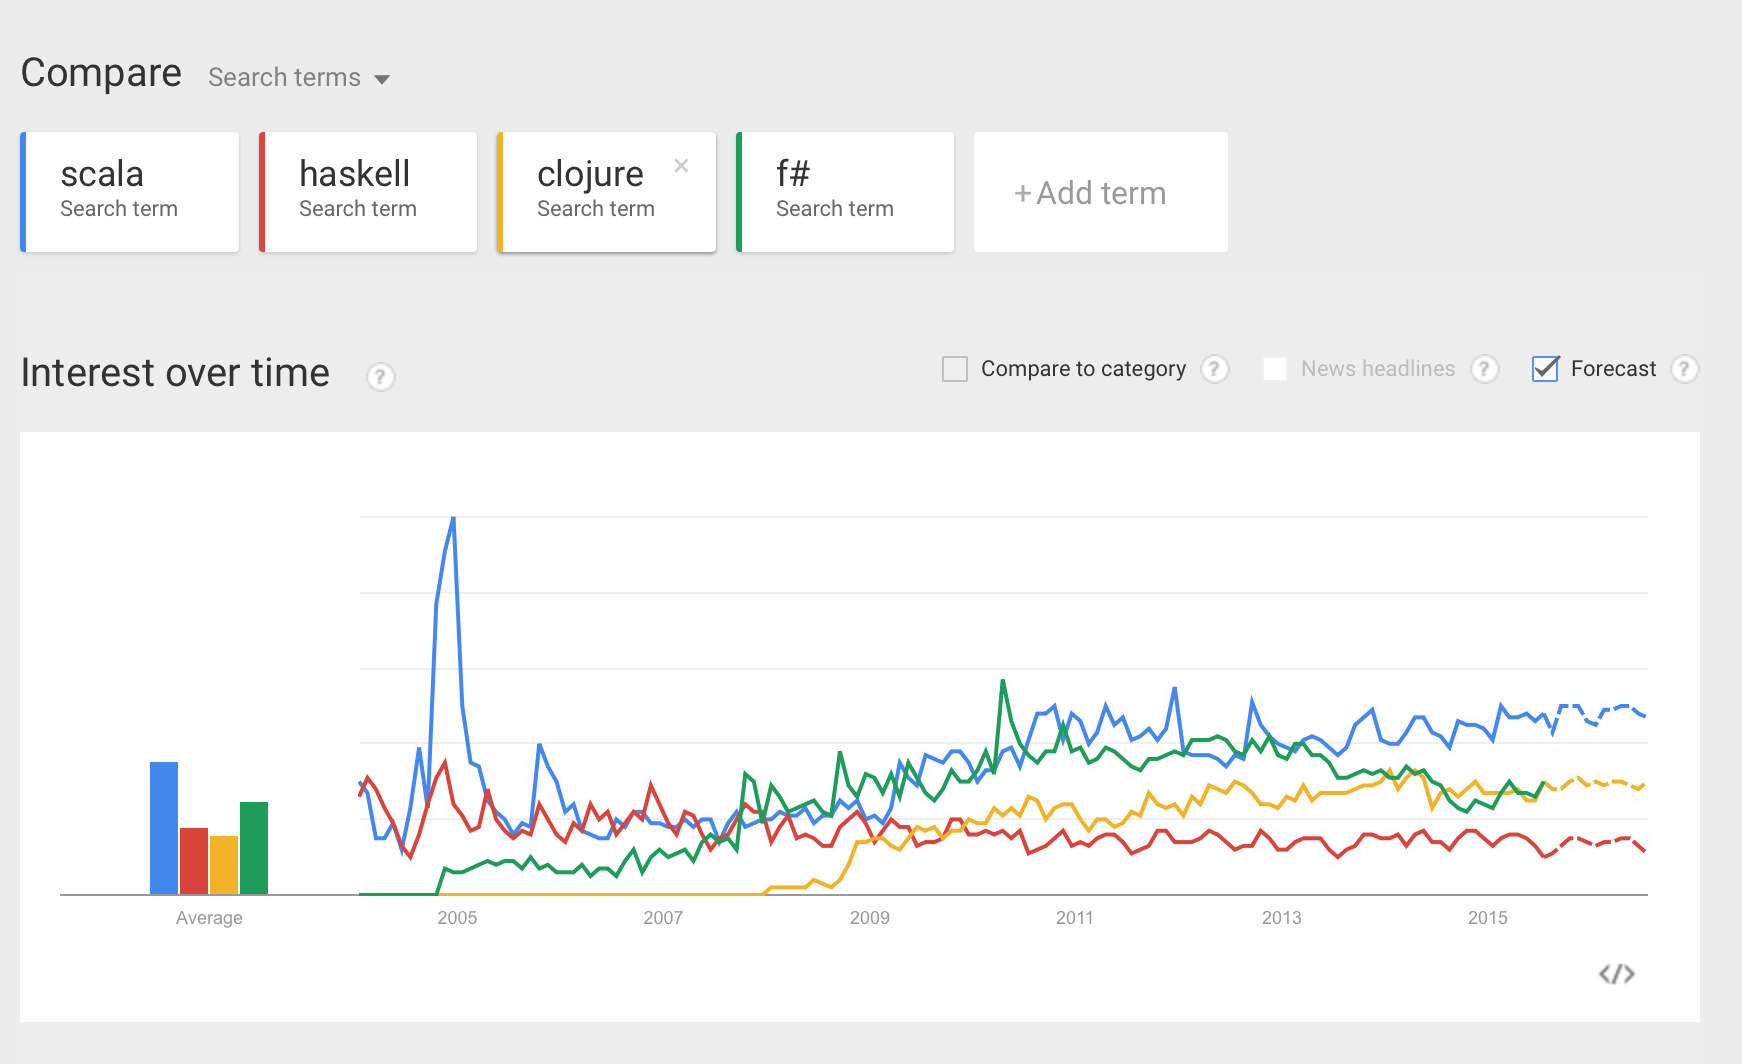
\includegraphics[width=\linewidth]{google-trends.png}
  \caption{Google search hits for programming languages - 2004 to July, 2015 }
  \label{fig:google-rank}
\end{figure}

Scala is one of the leading functional programming languages, over the last couple of years being adopted by large companies such as  Twitter(2009), Linkedin(2010), The Guardian, Foursquare. If we look at 'RedMonk Programming Languages Rankings'\cite{redmonk:1}, which is based on StackOverflow and Github analysis,  Scala occupies a worthy 14th position, being the first FP language in top . \par

\begin{figure}[h!]
  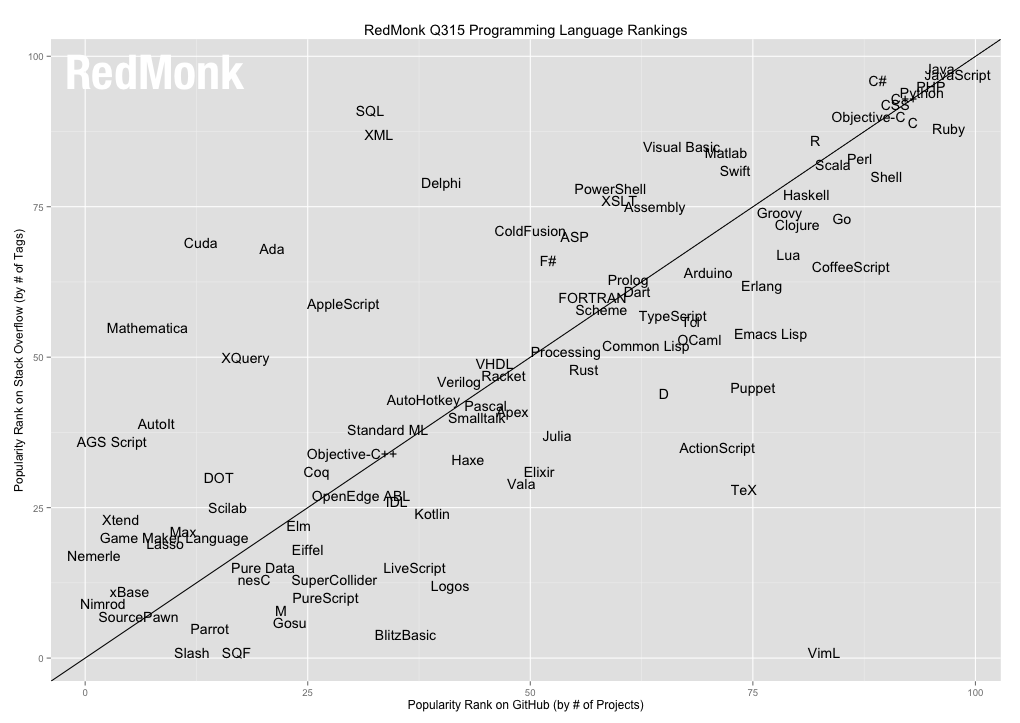
\includegraphics[width=\linewidth]{redmonk-rank.png}
  \caption{Redmonk rank of programming languages - June, 2015}
  \label{fig:redmonk-rank}
\end{figure}

One of its success factors is  Scala's compatibility with Java Virtual Machine hence code interoperability with Java, and the benefits that come along from  Java's well-established ecosystem. Another one might be that MOOCs  like Functional Programming in Scala \cite{scalastat:1} held  by the creator of Scala, Martin Odersky and Reactive Programming are one of the most popular online courses; the feedback from developers is really encouraging(see figure \ref{fig:interest}). \par

\begin{figure}[h!]
  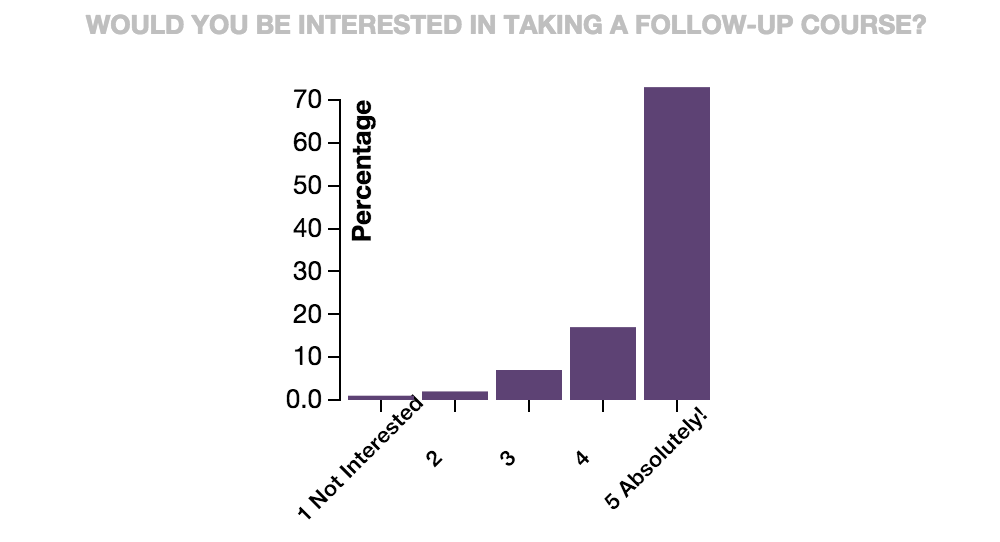
\includegraphics[width=\linewidth]{interest.png}
  \caption{Feedback FP in Scala course - interest in future courses on Scala (FP)}
  \label{fig:interest}
\end{figure}

Another reason why FP comes in handy nowadays is that multiprocessor architectures become ubiquitous and developers need to get more familiar with distributed and multi-threaded computing; programming with shared state has proven to be pretty difficult to reason about and functional programming offers to save a lot of headaches by removing shared state from the equation and providing better concurrency abstractions (Futures, Actors) and we should also consider  the exceptional distribution capabilities of map-reduce that FP offers. Although the programming paradigm was born more than 80 years ago, FP seems like a totally new way of thinking about software to modern day developers, having lots of secret gems left to be discovered. \par

\section {Problem statement}
Scala is a hybrid programming lanaguage being both a functional language and an object oriented one \cite{scalalang:1}.Writing Scala code does not imply you are writing functional code;  there is no mechanism in the language that enforces a functional style of programming; so one can say he writes code in Scala so he uses FP when in fact his code base is entirely procedural. I was also put in such a position,  being one of the many  developers that  switched from an Object Oriented language(Java /C\#/C++xs etc.)  to a functional language such as Scala. So how can one figure out if his Scala code follows the FP principles or not? The classic approach is to ask a functional programming expert for code review, if you are lucky enough to have access to such valuable resources. \par

The solution we propose is a set of metrics that should be able to quantify to what degree the code is making use of the functional paradigm. But what  qualifies a code as being functional? What are the specifics of a functional code? These are some of the questions that we have to answer first, in order to come up with metrics for code functional-ness.\par

\section {Theoretical Foundations}
First of all we need to establish the characteristics of FP languages, taking Scala as an example. Only then we can elaborate further on the metrics and decide which ones are to be considered for the study. \par

We get to ask ourselves the following questions: `how much does a method uses functional programming concepts?` Does it contain only immutable data, so no shared state? Does it use higher order functions for data processing? Does a method use advanced features such as monadic comprehension? Does a method use functional-like constructs such as anonymous inner classes? \par

\subsection {Immutability}
If a variable/object is immutable then it's value never changes. That is a really usefull guarantee if one plans on going concurrent: any such value can be safely shared amongst treads since the value is read-only. Another advantage is the reduced aliasing between different parts of the program; one can say that immutable objects are easier to reason about and also their API is straight forward because you don't need to reason about internal state changes - everything is transparent compared to mutable objects that introduce opaqueness in reasoning about their possible states at different moments of time . \par
Scala encourages immutability through case classes, which provide a syntatic sugar for creating immutable objects (data structures). Case classes are regular classes which export their constructor parameters and which provide a recursive decomposition mechanism via pattern matching.

\begin{lstlisting} 
abstract class Pet
case class Dog(name:String) extends Pet 
case class Cat(name:String) extends Pet
case class Hippo(name:String, weight:Int) extends Pet

//Decomposition
def printPetType(pet:Pet): String= pet match{
  case Dog => "it's a Dog"
  case Cat => "it's a Cat"
  case Hippo => "it's a Hippo"
}
\end{lstlisting}

By default, case classes ar immutable but one can change some of fields to be mutable, although it is not recommended.\par

Declaring a variable as a 'val' prevents it for being reassigned; still, this doesn't guarantee that the object it is reffering to is immutable. Best transparency is obtained with using both val's and immutable objects: this is the recommended approach also when dealing with concurrency. Scala provides both mutable and immutable collections that can be found in packages scala.collection.mutable and scala.collection.immmutable repectively. By default, Scala always picks immutable collections. 

\begin{lstlisting} 
val x = 4
x = 5 //Reasignment to val generates error
\end{lstlisting}


So, in order to create an immutable Scala object, it is necessary to have all the fields declared as vals + all the values to be immutable objects in turn. Case classes make it more easier to accomplish that in as few lines of code as possible.

\subsection {Referential tranparency, pure functions}
An expression is referentially transparent (RT) if it can be replaced by its resulting value without changing the behavior of the program. This must be true regardless of where the expression is used in the program. Programming without side effects leads to referential transparency. An example:

\begin{lstlisting}
def f(x:Int)= x* 3
val z = f(3)
\\Now, whenever we use z in the code, we can safely
\\ replace it with f(3) without changing the result of the program
\end{lstlisting}

Pure functions evaluates to the same result given the same argument value(s) and they don't have any side effects. A better definition can be found in 'Functional Programming in Scala' by Chiusano and Bjarnason : 'A function f is pure if expression f(x) is referentially transparent for all referentially trasparent values x'.\par
Examples of pure functions in Scala include:
\begin{itemize}

 \item Methods on immutable collections such as map, drop, filter, take
 \item Methods like split, length on the String class
 \item Mathematical functions such as add, multiply \ldots
\end{itemize}
As a rule of thumb in Scala if a function has its return type Unit, then most probably it has side effects. \par

A simple description for referential transparency would be expressed as:  \par
\begin{center}
\begin{math}
  RTI = \frac{ | \{ m \in M / Pure(m) \} | } { | M | }
\end{math}
\end{center}

Where  M - set of all functions/methods of the software and  Pure(m) - predicate that says if a function is pure or not. In this case, a value close to 1 corresponds to improved referential transparency while one close to 0 says that the property is not satisfied at all. \cite{DBLP:conf/icse/MudduABP13} \par

\subsection {High-order functions}
One of the features pointed out by John Hughes \cite{DBLP:journals/cj/Hughes89} in 'Why Functional Programming Matters' are higher- order functions and lazy evaluation; Hughes argues that these two concepts greatly increase the modularity of software by providing novative ways (compared to other structured programming techniques) of 'gluing' modules together so programs can become more concise and easier to reason about. One other design pattern that was first approached in Haskel and targets modularity by emphasizing on composition is represented by monads which model the concept of a category (see \ref{monads}). \par 
Before we begin talking about high-order functions we should first understand what does an order of a function mean:

\begin{itemize}
\item Order 0: Non function data
\item Order 1: Functions with domain and range of order 0
\item Order 2: Functions with domain and range of order 1
\item Order k: Functions with domain and range of order k-1
\end{itemize}

So order 0 is represented by numbers, lists, characters, etc. Order 1 are functions wich work with order 0 data. So order 1 data are the well known functions that every programming language supports. 
Functions with an order grater than 1 are callled higher-order functions and they fall at least in on of the following categories:
\begin{itemize}
\item they take other functions as parameters
\item they return a function as a result
\end{itemize}

An example is the following apply function written in Scala, which takes a function (defined on integers that returns a string) and an integer as parameters and returns the function application over the integer value: \par

\begin{lstlisting} 
def apply(f: Int => String, v: Int) = f(v)
\end{lstlisting} 


Classical higher-order functions over lists :

\begin{itemize}
\item Mapping: Application of a function on all elements in a list
\item Filtering : Collection of elements from a list which satisfy a particular condition
\item Accumulation: Pair wise combination of the elements of a list to a value of
another type
\item Zipping: Combination of two lists to a single list
\end{itemize}
[http://people.cs.aau.dk/~normark/prog3-03/pdf/higher-order-fu.pdf]

A study about high-order functions metrics and their corelation with software modularity was also conducted by B. Muddu et. al. \cite{DBLP:conf/icse/MudduABP13}. The proposed metric was studying the coupling between high order functions in diferent modules. It might be useful to make use also of their modularity metric when assesing code functional-ness.\par 

\subsection {Monads}  \label{monads}
In Category Theory, a Monad is a functor equipped with a pair of natural transformations satisfying the laws of associativity and identity. In Scala, monads are just a parametric type M[T] with two operations, flatMap (or bind) and unit which also preserves associativity and identity. \par

\begin{lstlisting}
trait M[T]{
  def flatMap[U](f:T=>M[U]): M[U]
}

def unit[T](x:T): M[T]
\end{lstlisting}

\subsection {Lazy evaluation}
Lazy evaluation or call-by-need is the opposite of eager evaluation(call-by-value) and it is an evaluation strategy which delays the evaluation of an expression until it is needed and only then computes the result and caches it for further evaluations. \par
One advantage is the memory saving due to postponing the evaluation but it comes with a performance cost: you get faster intialization but later (when evaluation occurs) you suffer a performance penality.\par

Scala supports laziness by introducing the lazy keyword and call by name parameters. By default it supports strict evaluation in contrast with Haskell which is lazy by default.

\begin{lstlisting}
lazy val product = 100 * 30 // not evaluated
println(product.toString) // evaluated 


object Test {
   def main(args: Array[String]) {
        delayed(time());
   }

   def time() = {
      println("Getting time in nano seconds")
      System.nanoTime
   }
   def delayed( t: => Long ) = {
      println("In delayed method")
      println("Param: " + t)
      t
   }
}

\end{lstlisting}

\section {State of the art - Literature study}
In the first section we talked about elaborating a series of metrics, in order to asses one's code functional-ness but we didn't had the opportunity to provide a proper definition for the concept of a metric and it's status quo in software industry. So metrics offer a quantitative measure of a software property. 

\subsection{Metrics}

\textit{"When you can measure what you are speaking about and express it in numbers, you know something about it; but when you cannot measure it, when you cannot express it in numbers, your knowledge is of a meagre and unsatisfactory kind: it may be the beginnings of knowledge but you have scarcely in your thoughts advanced to the stage of Science." (Lord Kelvin)}\par \par

A metric is a measurement function, and a software quality metric is "a function whose inputs are software data and whose output is a single numerical value that can be interpreted as the degree to which software possesses a given attribute that affects its quality \cite{Kaner04softwareengineering}. To some extent, metrics could be regarded as compiler warnings, signaling that a part of your code needs more testing. Software metrics are used in Software Engineering for helping with software development activities such as testing and refactoring, performance optimization, debugging, cost estimation, etc. Some common software metrics include : source line of code (LOC), number of functions, cyclomatic complexity, code coverage, cohesion, coupling. The most difficult part is not finding the code metrics but establishing a correlation between code metrics and process developing metrics. \par

Study of software metrics has been an active area of research since early 70' targeting mostly object oriented and imperative languages \cite{RyderT05:TFP_2005_Intellect}; as for functional languages, the number of published papers is not the numoerous; some of the prior work on metrics for functional languages was started almost 20 years ago by K. van den Berg in 1995 \cite{DBLP:journals/infsof/BergB95} who proposed a set of metrics for evaluating code complexity of Miranda functional programming language and Harrison which studied code modularity for SML \cite{eps250597}; 10 years later, Ryder and Thompson proposed some metrics for Haskell \cite{RyderT05:TFP_2005_Intellect} whereas  Muddu et. al. developed metrics for Scala \cite{DBLP:conf/icse/MudduABP13}. We can corelate the few number of papers on FP with the fact that FP does have yet such large adoption in software industry compared to object oriented and imperative languages. \par

Most commonly used metrics for functional languages in the papers we mentioned about are:

\begin{itemize}
\item Pattern related metrics - applies mostly to Haskell
\item Scoping metrics -how many scopes does a function introduce, the number of declatations brought in scope
\item Call graph metrics - strong connections, in degree, out degree, depth, width, arc-to-node ratio
\item Function atributes - path count, number of operands vs operators
\end{itemize}

The biggest problem with code metrics is not the definition of new ones but the extraction of  meaningful information from them;code metrics without semantics attached to them are just plain numbers; we need to corelate them to some process development metrics and this is the hardest part, since process activities are difficult to cuantify; most of the research in FP metrics is targeting maintanability, code quality and refactorings.  \par

In oder to study the maintability, Basavaraju Muddu et. al. introduce a technique for breaking software into logical modules \cite{DBLP:conf/icse/MudduABP13} The technique they chose was Modularizing by  Inverse-Depth heuristic, which is based of the project's file directory structure; they start at the source root folder and compute for each branch the maximum depth; then starting from the bottom up, they assign a module up to a certain depth; in their study, they use inverse depth of 1 for selecting modules, arguing that these are the closest approximation to actual logical modules. We would like to try other modularization techniques: package based, SBT (Scala Build Tool)  modularization and relate them to our problem: establishing code functional-ness: would a good 'functional-ness' value for our proposed metric lead also to improved modularity?.\par

\subsection {Static analysis tools for Scala}
There are already a couple of static analysis tools written for Scala : ScalaStyle, ScapeGoat, Wart remover, Linger and Scala Abide. These tools are looking possible errors that might appear in Scala code and also checks for a certain style of coding. Some of the checks they perform are: identation, illegal imports, multiple declared strings, null appearances, redundant if statements, cyclomatic complexity, unreachable catch statements, unexpected recursive definitions, unassigned variables, shadowing etc. \par

Some metrics that could turn out to be useful for our study are  the presence, absence of vars and cyclomatic complexity; ScalaStyle checks that classes and objects do not define mutable fields and that functions do not define mutable variables (VarFieldChecker, VarLocalChecker) \cite{scalastyle} and it also has a metric for cyclomatic complexity. At least from an implementation perspective it would be worthwhile to take them into account.\par

\section{Proposed solution}

We would like to try other modularization techniques: package based, SBT (Scala Build Tool)  modularization and relate them to our problem: establishing code functional-ness: would a good 'functional-ness' value for our proposed metric lead also to improved modularity?. [Basavaraju Muddu]\par

[FROM Muddu ] The system that we designed for Scala relies on the scalac compiler for source code parsing. We developed a plugin to the scalac compiler to visit the AST (Abstract Syntax Tree) created by the compiler. This extracts code metadata like classes, methods, parent-child relationships, method calls, etc., and stores it in a database (MySQL)

The other metrics presented by Muddu et. al. could be of further use if we decide to consider in our analysis also the software modularity ratio and try to establish correlation. As for the rest of the functional properties described in the previous section, we need to figure ourselves some proper metrics for them.

Scala provides an API to extend its compiler through Scala compiler plugins; how they work is that they insert custom functionality at different stages of the compilation; of course this could lead to errors, if used improperly. Unfortunately, there are only a limited amount of resources online (http://lampwww.epfl.ch/~magarcia/ScalaCompilerCornerReloaded/) that talk about how to create plugins. Muddu et. al. also used the scalac compiler to implement modularity metrics in Scala, gaining access to the AST representation of the source code \cite{DBLP:conf/icse/MudduABP13}.\par
We have to first decide upon the patterns that are most relevant and study about the compiler support for performing such analysis (Scala compiler plug-ins). 

\section{Conclusion}


\newpage


\bibliography{citation} 
\bibliographystyle{alpha}

\end{document}





